\chapter{Mass, Weight, and Gravity}
Mass is a measure of the amount of matter in an object. Weight is the force of gravity on that object. An object's mass is the same no matter where it is in the universe: the amount of ''stuff" in an object does not depend on its location. However, an object's weight \textit{does} change: the same object has a different weight on the Moon than it does on Earth or Venus. Since the force of gravity on the Moon is about $1/6^{th}$ as on Earth, you would weigh $1/6^{th}$ as much on the Moon, but your mass would be the same. 

\section{Kilograms versus Pounds}
In elementary school, you probably learned that 1 kilogram is about 2.2 pounds. This is only true \textit{on Earth}. In everyday language, we may use kilograms and pounds, or mass and weight, interchangeably; scientists do not. 

\begin{tabular}{|c|c|}\hline
\textbf{Mass} & \textbf{Weight}\\\hline
measure of \textit{amount} & measure of \textit{force}\\\hline
units include grams, kilograms, milligrams & units include pounds, Newtons, dynes\\\hline
a \textit{scalar} measurement & a \textit{vector} measurement\\\hline
does \textit{not} depend on location & does depend on location\\\hline
\end{tabular}

On Earth, a 1 kilogram mass weighs 2.2 pounds. That same mass weighs 0.37 pounds on the Moon. You learned to ''convert" between pounds in kilograms in elementary school because everywhere on Earth, a 1-kg mass weighs 2.2 lbs. The conversion doesn't apply to other locations in the universe because mass and weight are different. 

\subsection{Scalars and Vectors}
One of the fundamental differences between mass and weight is the type of measurement: scalar versus vector. \textit{Scalar} measurements are just a counting number: they tell the amount of magnitude. Mass is a scalar measurement: it tells how much matter is in an object. Energy is also a scalar measurement, as well as temperature and density. \textit{Vectors}, on the other hand, also have a \textit{direction}. A complete measure of a force gives the magnitude and direction. So, your weight isn't just 185 pounds: it's 185 pounds \textit{downward}. Velocity is a speed plus a direction, such as 35 mph east. We will expand on this later in the vectors chapter!

\section{Mass and Gravity}
When we discuss weight, we usually mean the gravitational force between an object and the largest nearby object. My weight on Earth, a spacecraft's weight on the Moon, or a rover's weight on Mars are all examples. But planets and moons don't have some special property that makes them emit gravity. Rather, \textit{all objects with mass are gravitationally attracted to each other}. But, compared to the mass of the Earth, the mass of all the other objects around you (a table, your family, your house or apartment complex) is very very small. 

The
force of the gravitational attraction between two objects is proportional to the product
of their masses, and inversely proportional to their distance squared.
This means that as objects get farther away, the force decreases. If you double the distance, the force quarters. Quadruple the distance, the force is $1/16^{th}$ as much. 
This is why you are more attracted to the earth than you are to
distant stars, even though they have much more mass than the earth.

\begin{mdframed}[style=important, frametitle={Newton's Law of Universal Gravitation}]

Two masses ($m_1$ and $m_2$) that are a distance of
$r$ from each other are attracted toward each other with a force of
magnitude:

$$F = G\frac{m_1 m_2}{r^2}$$

where $G$ is the universal gravitational constant. If you measure the
mass in kilograms and the distance in meters, $G$ is about $6.674
\times 10^{-11}$. That will get you the force of the attraction in
newtons.

\end{mdframed}

\textbf{Example}: %gravitational attraction between two regular objects

\begin{Exercise}[title={Gravity}, label=gravity_earth]

  The earth's mass is about $6 \times 10^{24}$ kilograms.

  Your spacecraft's mass is 6,800 kilograms.

  Your spacecraft is also about 100,000 km from the center of the earth. (For 
  reference, the moon is about 400,000 km from the center of the earth.)

  What is the force of gravity that is pulling your spacecraft and the earth 
  toward each other?

\end{Exercise}
\begin{Answer}[ref=gravity_earth]

  $$F = G\frac{m_1 m_2}{r^2} = (6.674 \times 10^{-11})\frac{(6.8 \time 10^3)(6 
  \times 10^{24})}{(10^5)^2} = 6.1 \times 10^{6}$$

  About 6 million newtons.

\end{Answer}

\section{Mass and Weight}

Gravity pulls on things proportional to their mass, so we often
ignore the difference between mass and weight.

The weight of an object is the force due to the object's mass and
gravity. When we say, ``This potato weighs 1 pound,'' we actually mean
``This potato weighs 1 pound on earth.'' That same potato would weigh
about one-fifth of a pound on the moon (see figure \ref{fig:massvweight}).

\begin{figure}[htbp]
\centering
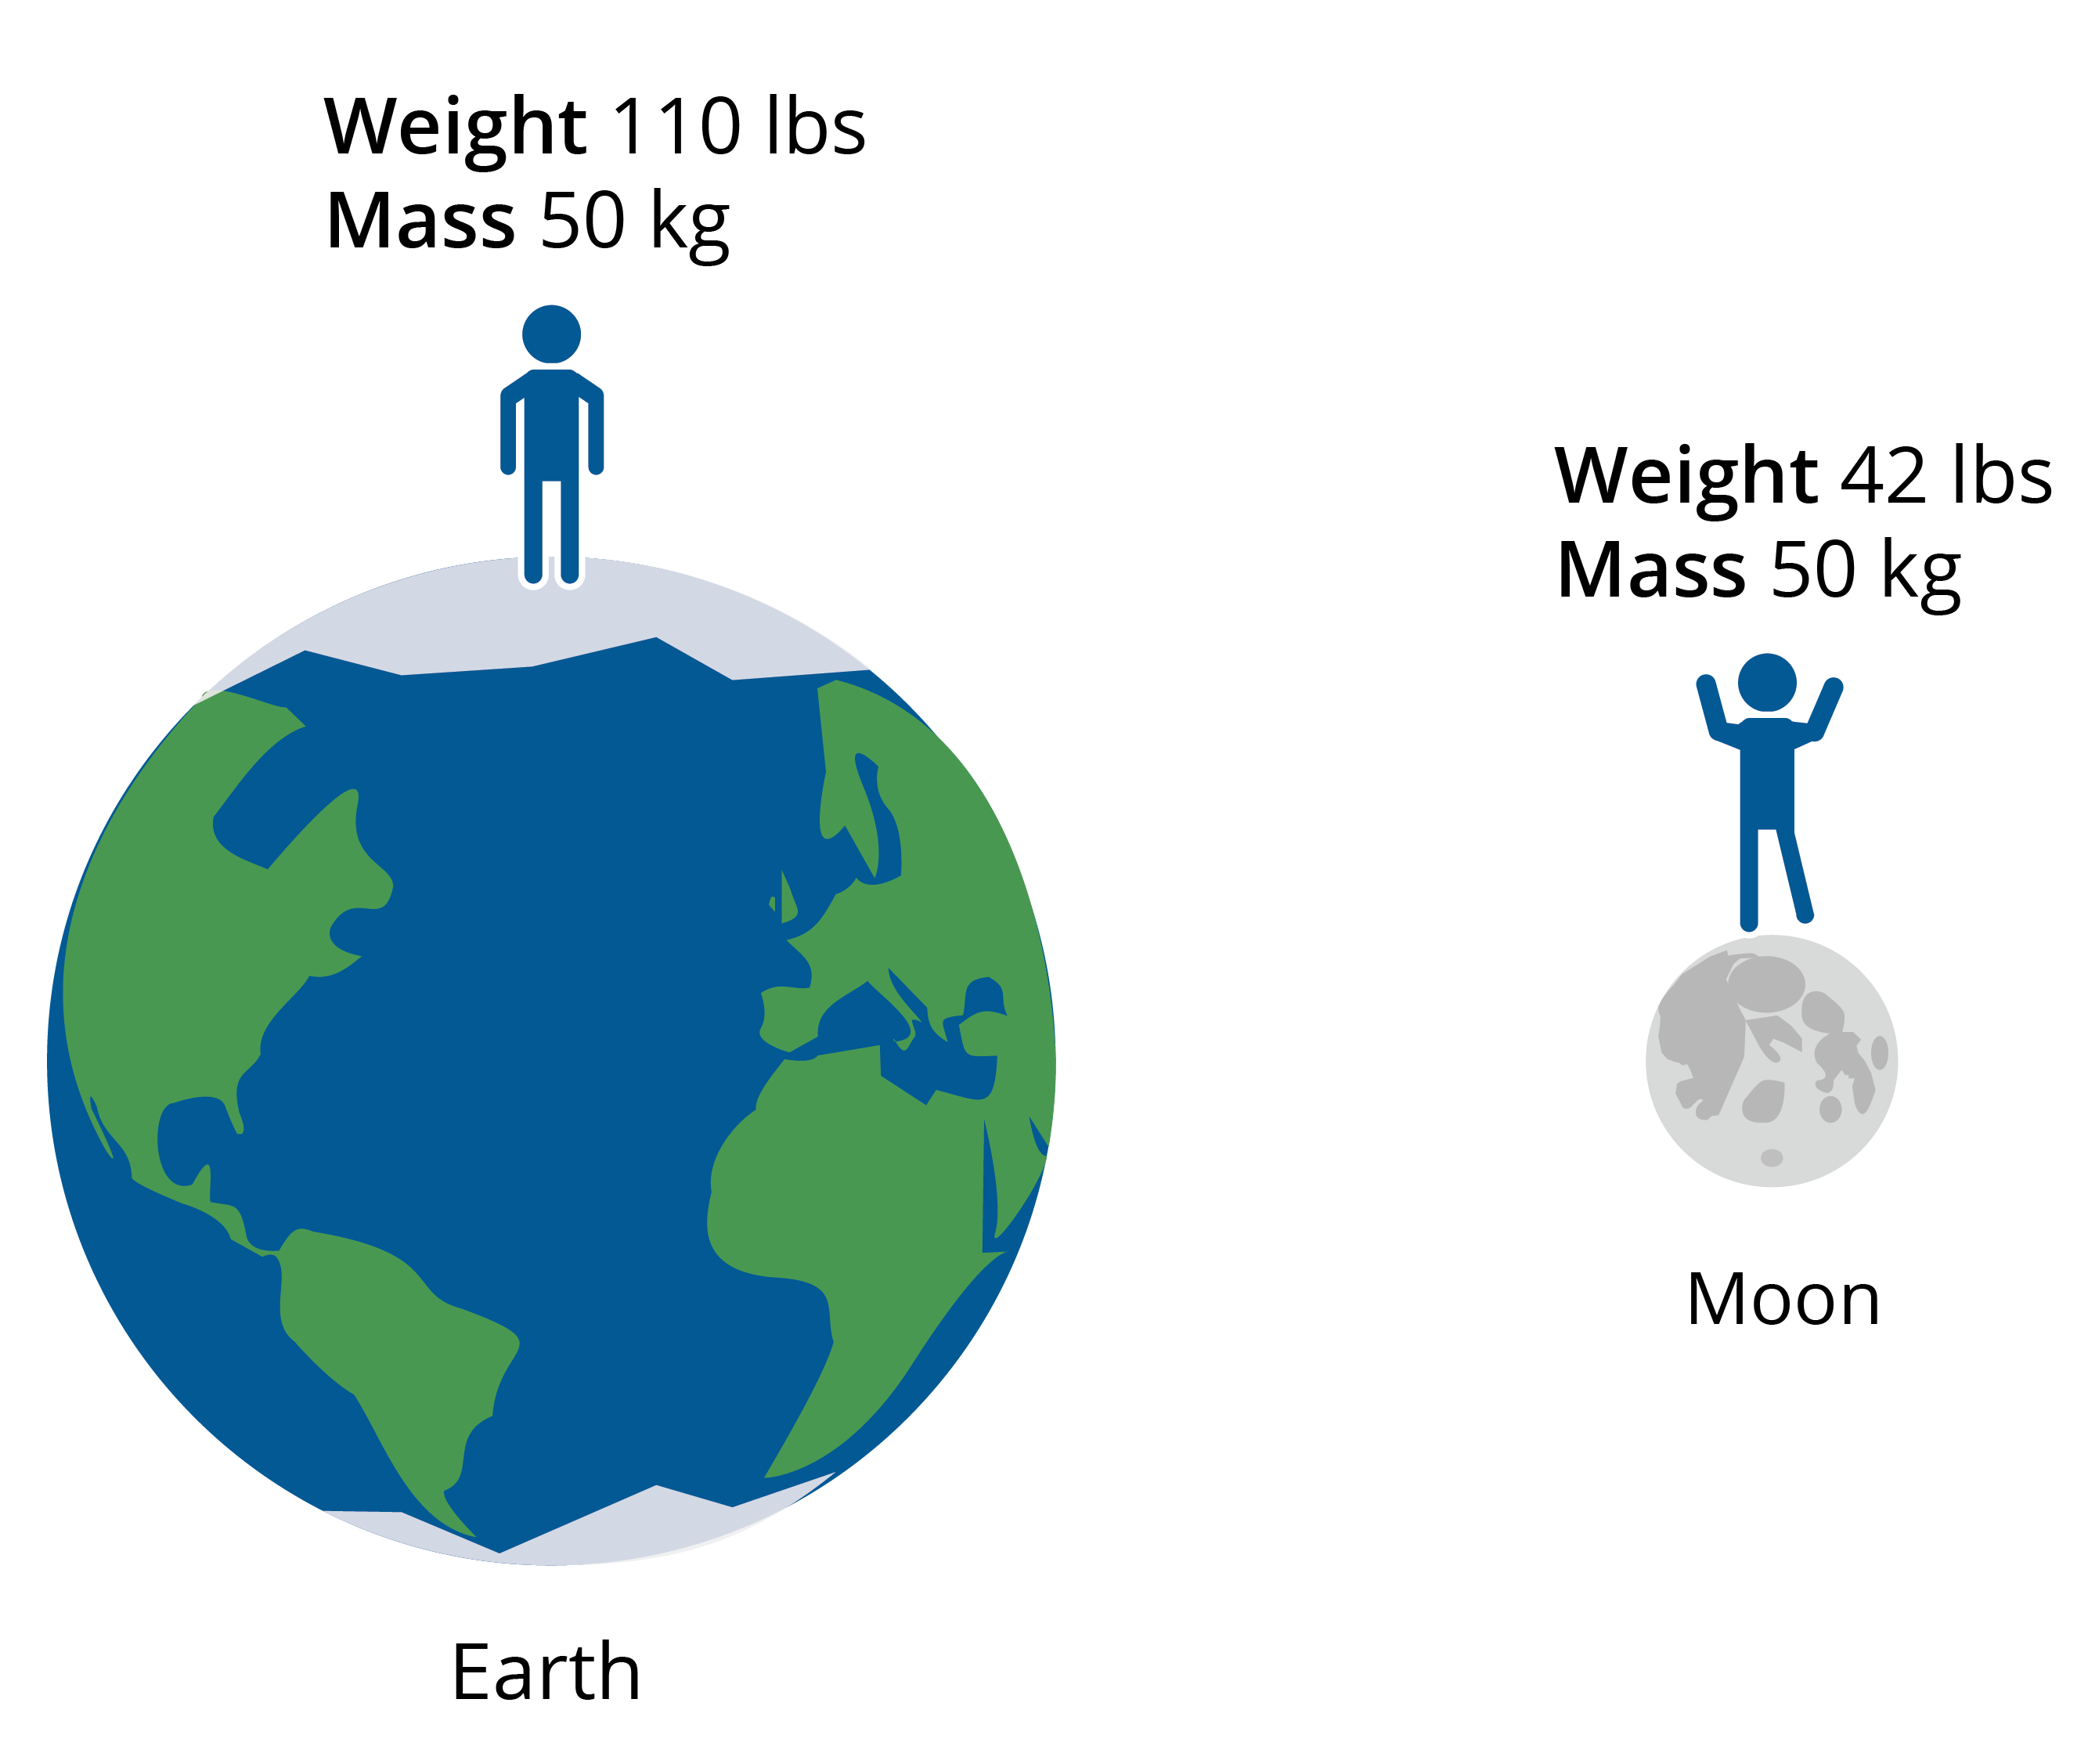
\includegraphics[width=0.7\textwidth]{massvweight.png}
\caption{Mass is a measure of all the matter in an object. Weight is a measure of 
the force of gravity on that object. Mass is not location-dependent, while weight 
is.}
\label{fig:massvweight}
\end{figure}

However, that potato has a mass of 0.45 kg no matter where it is in the universe.